\documentclass[12pt,a4paper]{article}
\usepackage[xetex]{graphicx}
\usepackage[no-math,silent]{fontspec}
\usepackage{xltxtra}
\usepackage[ancientgreek]{xgreek}
% footnote numbering starts with 1 for each page(perpage)
\usepackage{perpage}
%\setmainfont[{Mapping=tex-text}]{Times New Roman}
\setmainfont[{Mapping=tex-text}]{Times New Roman}
% No indented footnotes at the bottom of the page
\usepackage[bottom, flushmargin]{footmisc}
\MakePerPage{footnote}
\parindent=0in
%\newcommand{\gr}{\foreignlanguage{greek}}
\title{ΠΡΩΤΕΥΣ}
  \author{\tt {\small proteuss@sdf.lonestar.org}}
  \date{\grtoday}
% end title
\begin{document}
  \maketitle
  \begin{abstract}
    \noindent
    Ὁ Πρωτεὺς μετατρέπει κείμενα τῆς ἀρχαίας Ἑλληνικῆς
    καὶ Λατινικῆς γραμματείας ἅτινα διατίθενται κωδικευμένα ὑπὸ τὴν μορφὴν
    ὀπτικῶν δίσκων, γνωστῶν ὡς TLG καὶ PHI5/7. Διὰ τοῦ προγράμματος αὐτοῦ
    αἱ συλλογαὶ κειμένων διερευνῶνται ὡς πρὸς τὸ(ν) συγγραφέα/κείμενον καὶ
    ὁλόκληρα κείμενα μετατρέπονται εἰς μορφὴν pdf, unicode ἢ \LaTeX\ πρὸς
    ἐκτύπωσιν ἢ περαιτέρω ἐπεξεργασίαν.
  \end{abstract}
  \tableofcontents
\section{Εἰσαγωγή}
  Τὰ ἀρχαῖα Ἑλληνικὰ κείμενα τῆς ψηφιακῆς βιβλιοθήκης
  TLG\footnote{Thesaurus Linguae Grecae, ἤγουν Θησαυρὸς
               τῆς Ἑλληνικῆς Γλώσσης· εἶναι μία ἐκτενεστάτῃ
               συλλογὴ κειμένων τῆς ἀρχαίας Ἑλληνικῆς
               γραμματείας ψηφιακῶς κωδικευμένη. Ἡ συλλογὴ
               διατίθεται ὑπὸ μορφὴν ὀπτικοῦ δίσκου (CD-ROM).
               Ὅρα ἱστότοπον: http://www.tlg.uci.edu}
  καθὼς καὶ τὰ ἐπιγραφικά/παπυρικὰ καὶ Λατινικὰ κείμενα τῶν
  PHI\footnote{PHI εἶναι ἀρκτικόλεξον τοῦ Packard Humanities Institute.}
  CD5\footnote{ Τὸ CD5 εἶναι τὸ Λατινικὸν ἀνάλογον τοῦ TLG.
                Εἶναι δηλαδὴ μία σχεδὸν πλήρης
                συλλογὴ ὅλων τῶν Λατινικῶν κειμένων μέχρι τὸ 200 μ.Χ.
                Ἐπιπροσθέτως περιέχει καὶ βιβλικὰ κείμενα εἰς τὴν
                Ἑλληνικήν, Λατινικήν, Κοπτικήν,Ἑβραϊκὴν καὶ τὴν
                Ἀγγλικήν. Ὅρα:\\
                  {\scriptsize\tt
                https://web.archive.org/web/20170623105104/http://latin.packhum.org/canon}\\
                  {\scriptsize\tt
                  https://web.archive.org/web/20160803141809/http://www.indiana.edu/
                \textasciitilde letrs/text-tools/textlists/phibibliog.html }
              }
  καὶ PHI CD7\footnote{Τὸ CD7 περιέχει ἐκτενεστάτη συλλογὴ παπυρικῶν καὶ
                    ἐπιγραφικῶν κειμένων. Ἐνδιαφέροντα παραδείγματα εἶναι
                    τὸ Πάριον Χρονικόν, τὸ Χρονικὸν τῆς Μονεμβασίας καὶ οἱ
                    Ὀξυρρύγχειοι πάπυροι. Ὅρα ἱστότοπον:\\
                       {\scriptsize\tt https://web.archive.org/web/20080818140802/http://132.236.125.30/content.html }}
  δὲν εἶναι ἀπ᾽ εὐθείας ἀναγνώσιμα οὔτε ἐκτυπώσιμα καὶ χρειάζονται
  εἰδικὰ προγράμματα μετατροπῆς. Ὑπάρχουν
  προγράμματα\footnote{Diogenes, Musaios, Antiquarium κ.ἄ.}
  διερευνήσεως λέξεων ἢ φράσεων καὶ
  ἀποσπασματικῆς παρουσιάσεως τῶν συμφραζομένων ἄλλ᾽ οὐδὲν ἐξ αὐτῶν δύναται
  νὰ μετατρέψῃ ἐξ ὁλοκλήρου τὰ κείμενα τῆς ψηφιακῆς βιβλιοθήκης.
  Ὁ Πρωτεὺς εἶναι ἕνα πρόγραμμα ἀποκωδικεύσεως καὶ μετατροπῆς ὁλοκλήρων
  κειμένων. Τὰ κείμενα ἐξάγονται ὑπὸ τὴν μορφὴν Unicode
  (utf-8)\footnote{Ἐπεξεργάσιμα διὰ κειμενογράφων ὅπως ὁ Microsoft
  Office Word ἢ ὁ Libre/Open Office Writer.} ἢ κειμένου pdf.\footnote{Ἀναγνώσιμον
  καὶ ἐκτυπώσιμον διὰ τῶν Adobe Reader, kpdf, Evince κ.ἄ.} Διὰ τοῦ Πρωτέως
  εἶναι εὔκολος ἡ διερεύνησις τοῦ ὀνομαστικοῦ καταλόγου τῶν συγγραφέων
  καθὼς καὶ τῶν ὑπὸ ἕκαστον συγγραφέα περιεχομένων ἔργων.
  Ὁ Πρωτεὺς δὲν συνιστᾶται διὰ τὴν εὕρεσιν λέξεων ἢ φράσεων. Τὸ πλέον
  ἐνδεδειγμένο πρόγραμμα διερευνήσεως τῶν κειμένων εἶναι ὁ
  Διογένης,\footnote{\tt https://d.iogen.es/d/}
  ἐξ οὗ ὁ Πρωτεὺς μάλιστα ἤντλησεν προγραμματιστικὰς ἰδέας.
%%%%%%%%%%%%%%%%%%%%%%
% System Requirements
%%%%%%%%%%%%%%%%%%%%%%
\newpage
\section{Προδιαγραφαὶ Συστήματος}
  Ὁ Πρωτεὺς εἶναι ἕνα πρόγραμμα Perl
  ἀλλὰ διὰ λόγους ταχύτητος ἡ καρδιά του εἶναι γραμμένη
  σὲ ἁπλὴ C.\footnote{Ἡ ἐφαρμογὴ αὐτὴ (tlg2u) χρησιμοποιεῖται
              καὶ ἐκτὸς τοῦ Πρωτέως. Ὅρα εἰδικὸν ἐγχειρίδιον.}
  Διὰ τὴν τελικὴν στοιχειοθεσίαν τοῦ κειμένου pdf
  χρειάζεται τὴν \XeTeX.\footnote{Γλῶσσα προγραμματισμοῦ στοιχειοθεσίας,
                                    μέρος τοῦ συστήματος στοιχειοθεσίας
                                    \TeX.}
  Συνεπῶς ἀμφότεραι, Perl τε καὶ \XeTeX\, εἶναι ἀπαραίτητοι.
  Στοιχειώδεις ὁδηγίαι ἐγκαταστάσεώς των δίδονται
  κατωτέρω, ἀλλὰ καλὸν θὰ ἦτο νὰ συμβουλευθῆτε καὶ τὸ ἐγχειρίδιον τοῦ
  λειτουργικοῦ συστήματος.
  %
  \paragraph{Λειτουργικὸν Σύστημα.}
    Ὁ Πρωτεὺς ἔχει δοκιμασθῇ σὲ 64 bit Linux καὶ\newline
    Microsoft Windows. Τὰ ἀρχεῖα τοῦ προγράμματος καταλαμβάνουν ἐλάχιστον χῶρον (περὶ τὰ 3 Mb)
    σκληροῦ δίσκου· ἂν αἱ Perl τε καὶ \TeX\ ἀπουσιάζουν, τότε ἡ ἐγκατάστασίς
    των ἀπαιτεῖ ἕως καὶ 350 Mb.  Ἐπιπροσθέτως, ἐὰν τὰ κείμενα μεταφερθοῦν
    ἀπὸ τὰ CD εἰς τὸν σκληρὸν δίσκον, τότε θὰ ἀπαιτηθοῦν ἄλλα
    800\nolinebreak\ Mb.
  %
  \paragraph{Ὀπτικοὶ δίσκοι TLG καὶ PHI.}
    Πρέπει νὰ ἔχετε ἤδη τοὺς ὀπτικοὺς δίσκους μὲ τὰ κείμενα
    διότι ὁ Πρωτεὺς δὲν τὰ περιλαμβάνει.
    Τὰ ἐν ὀπτικῷ δίσκῳ κείμενα εἶναι ἀπ᾽ εὐθείας ἀναγνώσιμα ὑπὸ
    τοῦ Πρωτέως, καλύτερον ὅμως εἶναι τὰ ἀρχεῖα των νὰ μεταφερθοῦν εἰς
    κατάλογόν τινα τοῦ σκληροῦ δίσκου. Προτείνεται ἡ ἀκόλουθη διάταξις:
  \begin{verbatim}
              /usr/local/CDROMS/
                              |-- phi5
                              |-- phi7
                              |-- tlg
  \end{verbatim}
  %
  \paragraph{Perl.}
    Ἀπαραίτητος εἶναι ἡ Perl, ἐκδόσεως 5.8.6 ἢ μεταγενεστέρας,
    καθὼς καὶ τὰ πακέτα (modules) Perl-Tk, storable καὶ File-Slurp.
    Εἰδικῶς διὰ τὸ περιβάλλον Microsoft Windows, ἀπαιτοῦνται καὶ τὰ
    πακέτα Tk-Icon καὶ Win32-GUI.
  %
  \paragraph{\XeTeX.}
    Ἡ \XeTeX\ εἶναι μέρος τοῦ συστήματος ἠλεκτρονικῆς στοιχειοθεσίας
    \TeX\ οἷον καὶ πρέπει νὰ ἐγκατασταθῇ, καθὼς καὶ τὰ πακέτα
    (packages) «XeTeX», «latexmk», «xtab», «xgreek» (Ἑλληνικὸς συλλαβισμὸς
    καὶ Ἑλληνικὴ ἀρίθμησις) καὶ προαιρετικῶς τὸ πακέτο
    «philokalia» (βυζαντινοῦ τύπου γραμματοσειρὰ μὲ πλῆθος
    συντομογραφιῶν). Ἄνευ τοῦ \XeTeX\ ὁ Πρωτεὺς λειτουργεῖ
    ἀλλὰ περιορίζεται μόνον εἰς τὴν παραγωγὴν κειμένων unicode ἄνευ
    στοιχειοθεσίας.
  %
  \paragraph{Πολυτονικαὶ Γραμματοσειραὶ τύπου Unicode.}
    Τὸ λειτουργικὸν σύστημα δέον νὰ διαθέτη γραμματοσειρὰς Unicode
    τύπου «True Type» (ttf) ἢ «Open Type» (otf), αἵτιναι περιέχουν
    Ἑλληνικὰ στοιχεῖα στὶς θέσεις UCS 0370 - 03FF (Greek)
    καὶ UCS 1F00 - 1FFF (Greek Extended).
    Παραδεὶγματα καταλλήλων γραμματοσειρῶν εἶναι αἱ Palatino Linotype,
    Arial MS, Times New Roman, Tahoma κ.ἄ.
    Ἐξαιρέτους γραμματοσειρὰς παρέχει
    δωρεάν, μέσω τοῦ διαδικτύου, ἡ Ἑταιρεία Ἑλληνικῶν Τυπογραφικῶν
    Στοιχείων.\footnote{http://www.greekfontsociety-gfs.gr}
    Ἐπὶ παραδείγματι ἐξαιρετικῆς ποιότητος γραμματοσειραὶ εἶναι
    ἡ GFS Didot καὶ ἡ GFS NeoHellenic.
%
\section{Ἐγκατάστασις Linux}
  %%%%%%%%%%%%%%%%%%%%%%
  % Linux Installation
  %%%%%%%%%%%%%%%%%%%%%%
    Μεταφέρατε τὰ ἀρχεῖα τῶν TLG καὶ PHI ὅπως ἀναφέρεται ἀνωτέρω
    καὶ ἀποσυμπιέσατε τὰ ἀρχεῖα τοῦ Πρωτέως κάπου εἰς τὸν προσωπικόν σας
    κατάλογον (home directory).

    %
    \paragraph{\XeTeX.}
      Αἱ διανομαὶ Linux ἔχουν τὴν δυνατότητα εὐκόλου ἐγκαταστάσεως τοῦ
      \TeX.  Συνιστᾶται  ἡ ἐγκατάστασις τοῦ πλήρους TeX Live
      \footnote{http://www.tug.org/texlive/acquire.html}
      συμπεριλαμβανομένων ἁπάντων τῶν Ἑλληνικῶν πακέτων.
      Ἀπαραίτητα εἶναι τὰ πακέτα xetex, latexmk, xgreek, xtab καὶ προεραιτικῶς τὸ philokalia.
      Πρὸς ἐξακρίβωσιν τῆς δέουσας λειτουργίας τοῦ συστήματος στοιχειοθεσίας
      γράφομεν τὴν ἐντολήν: {\tt make xetex.tex} ἥτις θὰ ἐλέγξη αὐτομάτως
      τὸ σύστημα στοιχειοθεσίας καὶ ἂν ὅλα ἔχουν καλῶς,
      θὰ ἀναρτήσῃ ἐπὶ τῆς ὀθόνης μικρόν τι κείμενον pdf.
      Ἂν ἡ ἐντολὴ παρουσιάσῃ μηνύματα σφάλματος ἢ τὸ κείμενον
      τύχη κακέκτυπον, τότε ἐξετάζομεν προσεκτικῶς τὸ ἀρχεῖον
      ἀναφορᾶς (log file) {\tt \~{}test.log} καὶ ἀναθεωροῦμε
      τὴν ἐγκατάστασιν τοῦ \TeX\ κατὰ τὸ δέον.
    %
    \paragraph{Perl.}
      Ἅπασαι αἱ διανομαὶ Linux περιλαμβάνουν τὴν γλῶσσαν Perl,
      ὅμως καλὸν εἶναι νὰ βεβαιώσετε τὴν ὕπαρξιν ὅλων τῶν ἀναγκαίων
      πακέτων (modules). Πρὸς τοῦτο ἀνοίγουμε κονσόλαν ἐντολῶν (terminal)
      καὶ δίδομεν τὴν  ἐντολήν: {\tt sudo make perl\_test}.
    %
      \paragraph{Ἐγκατάστασις Γραμματοσειρῶν.} Διὰ τῆς ἐντολῆς {\tt sudo
      make fonts} ὁ Πρωτεὺς θὰ μεταφέρει γραματοσειράς τινας εἰς τὴν
      τοποθεσίαν\\ {\tt /usr/local/share/fonts} ὅθεν θὰ εἶναι διαθέσιμες καὶ
      ἀπὸ ἄλλες ἐφαρμογές.
    %
    \paragraph{Ἐγκατάστασις τοῦ Πρωτέως.}
      Γράφομεν τὴν ἐντολήν: {\tt sudo make install}.
      Ἡ ἐγκατάστασις θὰ γίνη εἰς τὴν θέσιν {\tt /usr/local/proteus}.
      Ἐὰν ἐπιθυμῆτε ἐγκατάστασιν εἰς ἄλλην θέσιν, τότε ἀλλάξατε τὴν τιμὴν
      τῆς μεταβλητῆς\\ {\tt INSTALL\_PREFIX} τῆς πρώτης σειρᾶς τοῦ ἀρχείου
    {\tt makefile}. Ἐπίσης ὁ Πρωτεὺς κατὰ τὴν ἐγκατάστασίν του θὰ μεταφέρη
      γραμματοσειράς τινας εἰς τὸν κατάλογον: {\tt /usr/local/share/fonts}.
      Μετὰ ταῦτα ὁ Πρωτεὺς εἶναι ἕτοιμος πρὸς χρῆσιν. Ἡ ἐκκίνησις γίνεται
      ἤτε διὰ εἰκονιδίου τοῦ μενοῦ Ἐνάρξεως (Start Menu) ἤτε διὰ ἐντολῆς
      κονσόλας ({\tt proteus}).
    %
    \paragraph{Καθορισμὸς καταλόγων.}
      Κατὰ τὴν πρώτην του ἐκκίνησιν ὁ Πρωτεὺς θὰ δημιουργήση κατάλογον
      {\tt \~{}/.proteus}, ὅπου θὰ καταγραφοῦν αἱ ρυθμίσεις τοῦ προγράμματος
      καθὼς καὶ τὰ παραχθέντα κείμενα. Ἴσως δὲ ζητήσει καὶ τὸν ἐντοπισμὸν τῶν
      ἀρχείων τῶν συλλογῶν TLG καὶ PHI5/7.
      Δώσατε τὴν θέσιν των ὅταν αὐτὸ ζητηθῆ.  Ὁ Πρωτεὺς καταγράφει τὴν πληροφορίαν
      ταύτην καὶ θὰ τὴν ζητήση ἐκ νέου μόνον εἰς περίπτωσιν
      ἀλλαγῆς τῆς θέσεως τῶν ἀρχείων.  Τὰ παραγόμενα ὑπὸ τοῦ Πρωτέως κείμενα, ἤτοι
      ἀρχεῖα .pdf καὶ .utf, ἀρχικῶς ἀποστέλλονται εἰς τὸν κατάλογον (subdirectory)
      {\tt \~{}/.proteus/books}. Ὁ προορισμὸς αὐτὸς δύναται νὰ τροποποιηθῆ
      διὰ τῆς γραμμῆς ἐπιλογέων (menu bar) καὶ τῶν κομβίων
      {\bf Files} καὶ {\bf Output Directory}. (ὅρα Σχῆμα 1.)
    %
    \paragraph{Ἀπεγκατάστασις.}
      Πλήρης διαγραφὴ τοῦ Πρωτέως ἐκ τοῦ συστήματος γίνεται διὰ τῆς ἐντολῆς:
      {\tt sudo make uninstal}.  Ἡ ἀπεγκατάστασις δὲν θὰ
      διαγράψη τὸν προσωπικὸν κατάλογον {\tt \~{}/.proteus}.
 %
    %%%%%%%%%%%%%%%%%%%%%%
    % Windows Installation
    %%%%%%%%%%%%%%%%%%%%%%
  %\subsection{Windows}
  %  Ἡ ἐγκατάστασις εἶναι ἁπλουστάτη.  Ἀποσυμπιέσατε τὰ ἀρχεῖα εἰς
  %  προσωρινὸν κατάλογον (ἢ μεταβῆτε εἰς τὸ CD) καὶ ἐκκινήσατε τὸ
  %  πρόγραμμα ἐγκαταστάσεως
  %  {\tt proteus-setup.exe}. Ὅ,τι χρειάζεται ὁ Πρωτεὺς θὰ ἐγκατασταθῆ
  %  αὐτομάτως.
  %  Ἐκκίνησις τοῦ Πρωτέως γίνεται ἤτε διὰ εἰκονιδίου τοῦ μενοῦ
  %  Ἐνάρξεως (Start Menu), Programs, Proteus,
  %  ἤτε διὰ ὁμωνύμου εἰκονιδίου τῆς επιφανείας ἐργασίας.
  %  %
  %  \paragraph{Καθορισμὸς καταλόγων.}
  %    Κατὰ τὴν πρώτην του ἐκκίνησιν ὁ Πρωτεὺς ἴσως ζητήσει τὸν ἐντοπισμὸν
  %    τῶν ἀρχείων τῶν συλλογῶν TLG καὶ PHI5/7.  Δώσατε τὴν θέσιν των
  %    ὅταν αὐτὸ ζητηθῆ.  Ὁ Πρωτεὺς καταγράφει τὴν πληροφορίαν
  %    ταύτην καὶ θὰ τὴν ζητήση ἐκ νέου μόνον εἰς περίπτωσιν
  %    ἀλλαγῆς τῆς θέσεως τῶν ἀρχείων.  Τὰ παραγόμενα ὑπὸ τοῦ Πρωτέως κείμενα, ἤτοι
  %    ἀρχεῖα .pdf καὶ .utf, ἀρχικῶς ἀποστέλλονται εἰς τὸν κατάλογον (subdirectory)
  %    \verb+C:\Program Files\proteus\books+.
  %    Ὁ προορισμὸς αὐτὸς δύναται νὰ τροποποιηθῆ διὰ τῆς γραμμῆς ἐπιλογέων
  %    (menu bar)
  %    {\bf Files} καὶ {\bf Output Directory}. (ὅρα Σχῆμα 1.)
  %  %
  %  \paragraph{Ἀπεγκατάστασις.}
  %    Πλήρης διαγραφὴ τοῦ Πρωτέως ἐκ τοῦ συστήματος γίνεται διὰ εἰκονιδίου
  %    τοῦ μενοῦ Ἐνάρξεως (Start Menu), Programs, Proteus, uninstall.
  %
  %%%%%%%%%%%%%%%%%%%%%%
  %       Usage
  %%%%%%%%%%%%%%%%%%%%%%
\section{Ὁδηγίαι χρήσεως}
  \subsection{Ἐντοπισμὸς κειμένων}
    \subsubsection*{Πίναξ συγγραφέων}
      Κατὰ τὴν ἐκκίνησίν του ὁ Πρωτεὺς παραθέτει
      κατάλογον συγγραφέων ὧν τὰ ἔργα περιέχονται ἐν τῆ συλλογῆ κειμένων
      καθοριζομένη διὰ τοῦ κομβίου {\bf Corpus}.
          \begin{figure}[htp]
            \begin{center}
              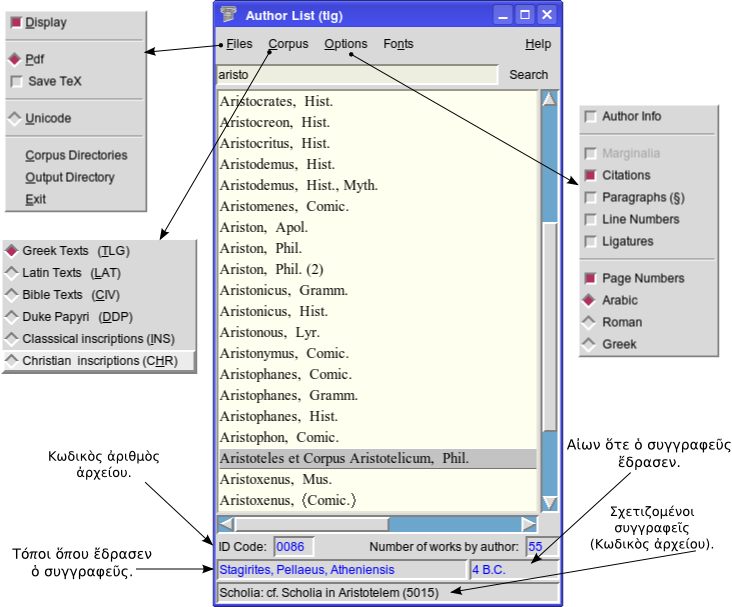
\includegraphics[scale=0.7]{../images/author-gr.png}
              \caption{Ὁ κατάλογος τῆς συλλογῆς TLG ἥτις
                      περιέχει πλέον τῶν 3.500 συγγραφέων.
                      Φαίνονται καὶ τὰ ἀναπτύγματα τῶν κομβίων
                      τῆς γραμμῆς τῶν ἐπιλογέων ({\small menu bar}).}
            \end{center}
          \end{figure}
    Τὸ ὄνομα οἱουδήποτε συγγραφέως εὑρίσκεται εὐκόλως διὰ τῆς γραφῆς ἐν τῆ
    γραμμῆ εὑρέσεως ὀλίγων ἐκ τῶν γραμμάτων τοῦ ὀνόματός του. Παρατηροῦμεν ὅτι ὁ
    κατάλογος ἀμέσως περιορίζεται εἰς συγγραφεῖς ὧν τὰ ὀνόματα περιέχουν τὰ
    γράμματα ἐν τῆ γραμμῆ εὑρέσεως.
    Π.χ. γράφοντες «{\tt herod}»\footnote{Δυστυχῶς τὰ ὀνόματα τῶν συγγραφέων
    ἐν τῶ TLG εἶναι Λατινιστί.} ὁ κατάλογος θὰ παρουσιάση μόνον τά:
    Herodianus, Herodas, Herodotus, ... κ.λπ.
    Ἂν γράψωμεν «{\tt lexic}» ὁ κατάλογος θὰ παρουσιάση ὅλα τὰ λεξικὰ τῆς
    βιβλιοθήκης.
    Ἡ γραμμὴ εὑρέσεως δέχεται καὶ κανονικὰς διατυπώσεις\footnote{Συχνάκις
    ἀπαντᾶται ὁ ὅρος «κανονικαὶ ἐκφράσεις».} (regular expressions).
    Π.χ. γράφοντες «{\tt \textasciicircum{}h.*tus}» ὁ κατάλογος θὰ  παρουσιάση
    μόνον τὰ Heraclitus καὶ Herodotus.
    %
  \subsubsection*{Πίναξ ἔργων συγγραφέως} Ἐπιλογή τινος ἐκ τῶν
    συγγραφέων\footnote{Διὰ τοῦ πληκτρολογίου (βέλη κατευθύνσεως, page up/down)
    ἢ διὰ τοῦ μυός.} θὰ παρουσιάση τὸν κατάλογον τῶν ἔργων του.
          \begin{figure}[htb]
            \begin{center}
              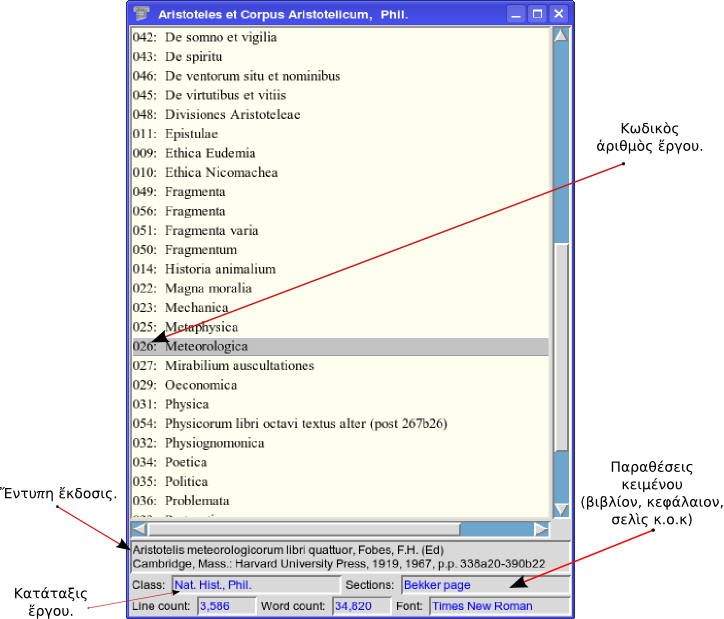
\includegraphics[scale=0.6]{../images/works-gr.png}
              \caption{Ὁ κατάλογος τῶν ἔργων τοῦ συγγραφέως.}
            \end{center}
          \end{figure}
    %
  \subsection{Μετατροπὴ εἰς unicode}
    Ἐκ τῶν στοιχείων τῆς γραμμῆς ἐπιλογέων (menu bar) διαλέξατε τὸν κατιόντα
    κατάλογον (drop down menu) {\bf Files} καὶ ἐξ αὐτοῦ τὸν
    τίτλον {\bf Unicode}.
    Ὅλα τὰ στοιχεῖα τὰ σχετιζόμενα μὲ τὴν μετατροπὴν εἰς .pdf
    ἀπενεργοποιοῦνται αὐτομάτως καὶ ἀποκτοῦν φαιὰν ὄψιν.

              \begin{figure}[htb]
                \begin{center}
                                        %% scale=l b r t
                  \fbox{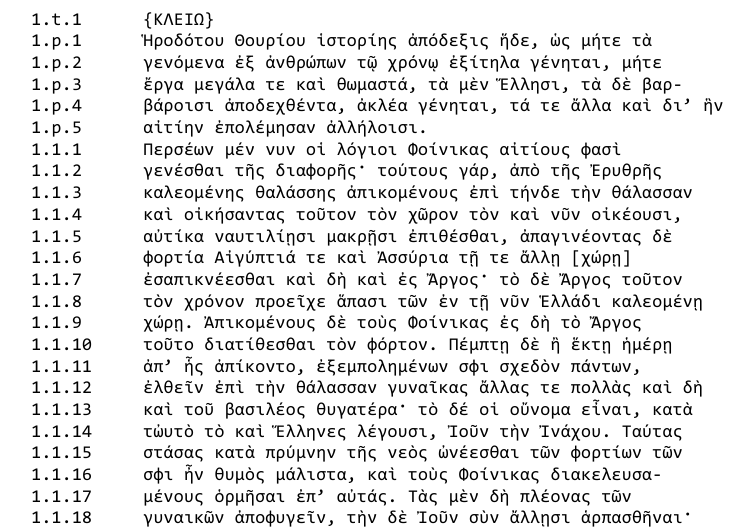
\includegraphics[scale=0.4]{../images/herod1.png}}
                    \caption{Παράδειγμα κειμένου utf-8 ὅπως ἐμφανίζεται
                           εἰς τὸν MS Word. Ἡ γραμματοσειρὰ εἶναι
                           ἡ ἰσοπαχὴς Consolas.
                           Ἀριστερόθεν φαίνονται
                           αἱ ἀριθμήσεις τοῦ κειμένου. Ὁ τίτλος
                           ἐμφανίζεται ἐντὸς ἀγκίστρων (\{\}) καὶ
                           σημειοῦται διὰ τοῦ  ``t'', ἐνῶ διὰ τοῦ ``p''
                           σημειοῦται τὸ προοίμιον.}
                \end{center}
              \end{figure}
    Πιέζοντες τὸ πλῆκτρον «Enter» (ἢ πιέζοντες δὶς τὸ
    ἀριστερὸν πλῆκτρον τοῦ μυός) ἐπί τινος ἐκ τῶν ἔργων τοῦ συγγραφέως,
    ἐκκινεῖ τὴν μετατροπὴν τοῦ κειμένου καὶ τὴν ἀποθήκευσίν του
    εἰς ἀρχεῖον μορφῆς Unicode.\footnote{Ἡ διάρκεια τῆς μετατροπῆς
                      ἐξαρτᾶται ἀπὸ τὸ μέγεθος τῶν ἀρχείων.
                      Ἐπὶ παραδείγματι τὸ ἀρχεῖον τῶν ἁπάντων
                      τοῦ Ἰωάννου τοῦ Χρυσοστόμου ἔχει μέγεθος
                      32 Mb καὶ περιλαμβάνει 402 συγγράμματα,
                      τὸ δὲ Ἀνθολόγιον τοῦ Ἰωάννου τοῦ Στοβαίου
                      περιέχει 1.260 σελίδες. Ἡ ἐξαγωγὴ καὶ
                      μετατροπὴ τέτοιων κειμένων πιθανὸν νὰ διαρκέση
                      μερικὰ λεπτά.}
    Ἐπίσης τὸ πρόγραμμα θὰ ζητήση ἕνα ὄνομα ἀρχείου, ἐνῶ θὰ προτείνη ὄνομα
    σχηματιζόμενον ἐκ τῶν κωδικῶν ἀριθμῶν τοῦ συγγραφέως καὶ τοῦ ἐπιλεχθέντος
    ἔργου. Συνιστᾶται ὅπως κρατηθῆ ἡ κατάληξις {\bf .utf}.
    Τὸ ἀρχεῖον ἀκολούθως θὰ διαβιβασθῆ αὐτομάτως
    (ἐὰν ἡ προαίρεσις {\bf Display} εἶναι ἐνεργός) εἰς τὸν κειμενογράφον πρὸς
    παρουσίασιν καὶ ἐπεξεργασίαν.\footnote{Ὁ Microsoft Word εἶναι ὀλίγον
                        ἀργὸς κατὰ τὴν ἐκκίνησιν.  Ἐπίσης, κατὰ τὴν πρώτην
                        φορὰν ὅτε τὰ Windows τυγχάνουν ἀρχείου μὲ κατάληξιν
                        {\bf .utf}, θὰ ἐρωτήσουν μὲ τί πρόγραμμα νὰ τὸ
                        συσχετίζουν ἐφεξῆς. Διαλέγουμε «Microsoft Office Word»
                        καὶ τὸ «Always use the selected program...»}
    Ἂν ζητηθῆ, εἰσάγομεν τὴν κωδίκευσιν (encoding) «Unicode (utf-8)» καὶ τὴν
    γραμματοσειρὰν τῆς ἀρεσκείας μας.\footnote{Μόνον διὰ τὸ Open Office Writer.}
    Τέλος, ὅταν ἀνοίξη ὁ κειμενογράφος, βάζουμε τὸ κείμενον εἰς Ἑλληνικὴν
    πολυτονικὴν γραμματοσειράν. (CTRL-A ἐπιλέγει ὁλόκληρον τὸ κείμενον).
    Ἐάν το κείμενον κατόπιν ἐπιλογῆς μας ἐνσωματώνει πληροφορίας εἰς τὰ
    περιθώρια (ἀριθμήσεις παραγράφων, στίχων κ.λπ.) συνιστᾶται ἡ χρῆσις
    ἰσοπαχείας γραμματοσειρᾶς (monospaced font)\footnote{
                                              π.χ. Consolas ἢ Courier}
    ὥστε νὰ διατηρηθῆ ἡ σωστὴ στοίχισις τοῦ κειμένου.
%  \newpage
    %
  \subsection{Μετατροπὴ εἰς Pdf}
    Ἐκ τῶν στοιχείων τῆς γραμμῆς ἐπιλογέων (menu bar)
    διαλέξατε τὸν κατιόντα κατάλογον {\bf Files}
    καὶ ἐξ αὐτοῦ τὸν τίτλον {\bf Pdf}.
    Ὅλα τὰ στοιχεῖα τὰ σχετιζόμενα μὲ τὴν
    μετατροπὴν εἰς .pdf ἐνεργοποιοῦνται αὐτομάτως.
    Πιέζοντας τὸ πλῆκτρον «Enter» (ἢ πιέζοντας δὶς τὸ
    ἀριστερὸν πλῆκτρον τοῦ μυός) ἐπί τινος ἐκ τῶν ἔργων
    τοῦ συγγραφέως, ἐκκινεῖ τὴν μετατροπὴν τοῦ κειμένου
    καὶ τὴν ἀποθήκευσίν του εἰς ἀρχεῖον μορφῆς pdf.
    Ἐπίσης τὸ πρόγραμμα θὰ ζητήση ἕνα ὄνομα ἀρχείου,
    ἐνῶ θὰ προτείνη ὄνομα σχηματιζόμενον ἐκ τῶν κωδικῶν
    ἀριθμῶν τοῦ συγγραφέως καὶ τοῦ ἐπιλεχθέντος
    ἔργου. Συνιστᾶται ὅπως κρατηθῆ ἡ κατάληξις {\bf .pdf}.
    Τὸ ἀρχεῖον ἀκολούθως θὰ διαβιβασθῆ αὐτομάτως (ἐὰν ἡ
    προαίρεσις {\bf Display} εἶναι ἐνεργός)  εἰς τὸν κατάλληλον
    ἀναγνωστῆραν (Adobe Reader, Kpdf κ.λπ.).
    Ἐνεργοποίησις τῆς προαιρέσεως {\bf Save TeX} δίδει ἐπιπροσθέτως
    ἀρχεῖον περιέχον τὸ κείμενον
    σὺν τὰς στοιχειοθετικὰς ὁδηγίας τοῦ \XeTeX· χρήσιμον διὰ
    τοὺς ἐπιθυμοῦντας νὰ ἀλλάξουν τὸ αὐτομάτως
    παραγόμενον pdf.\footnote{Παράδειγμα τέτοιας παρεμβάσεως
                              εἶναι το κείμενον τοῦ σχήματος 5.}
    Τὸ ὄνομα τοῦ ἀρχείου αὐτοῦ εἶναι {\tt file\_name.tex} καὶ ἡ
    στοιχειοθεσία ἐκτὸς Πρωτέως γίνεται τοιουτοτρόπως:
    {\tt xelatex file\_name.tex}.
    Ἡ αὐτόματος στοιχειοθεσία καθορίζεται ἐκ πολλῶν προαιρέσεων
    (options) αἵτιναι περιγράφονται κατωτέρω.
  %      Corpus
  \subsection{Ἐπιλογεὺς συλλογῆς κειμένων (Corpus)}
    Τὸ ὑπὸ τίτλον {\bf Corpus} κομβίον παραθέτει ἐπιλογέα
    διὰ τὰς ἑξῆς συλλογὰς κειμένων:
    \begin{itemize}
      \item{\bf Greek Texts: }Ἑλληνικὰ κείμενα  (TLG)
      \item{\bf Latin Texts: }Λατινικὰ κείμενα  (LAT)
      \item{\bf Bible Texts: }Συλλογὴ βιβλικῶν κειμένων Ἑλληνιστί,
                        Λατινιστὶ καὶ Ἀγγλιστὶ  (CIV)
      \item{\bf Duke Papyri: }Παπυρικὰ κείμενα ὡς ἐπὶ τὸ πλεῖστον
          Ἑλληνιστὶ (DDP)
      \item{\bf Classical Inscriptions: }Ἑλληνικαὶ καὶ Λατινικαὶ ἐπιγραφαὶ
          τῶν κλασσικῶν καὶ Ἐλληνιστικῶν χρόνων (INS)
      \item{\bf Christian Inscriptions: }Ἑλληνικαὶ καὶ Λατινικαὶ ἐπιγραφαὶ
          τῆς χριστιανικῆς περιόδου (CHR)
    \end{itemize}
    Τὰ ἐντὸς παρενθέσεως 3 γράμματα δηλώνουν τὸ πρόθεμα τοῦ ὀνόματος τῶν
    ἀρχείων ἑκάστης συλλογῆς. Ἐπὶ παραδείγματι, τὰ Ἑλληνικὰ ἀρχεῖα ἔχουν
    ὀνόματα τῆς μορφῆς tlgxxxx.txt, ἐνῶ τὰ βιβλικὰ κείμενα ἔχουν civxxxx.txt.
    Ὅπου, xxxx εἶναι ὁ τετραψήφιος κωδικὸς τοῦ συγγραφέως.
    Τέλος, τὰ LAT καὶ CIV εἶναι μέρος τοῦ PHI CD5, τὰ δὲ DDP, INS καὶ CHR
    εὑρίσκονται εἰς τὸ PHI CD7.
              \begin{figure}[htb]
                \begin{center}
                  \fbox{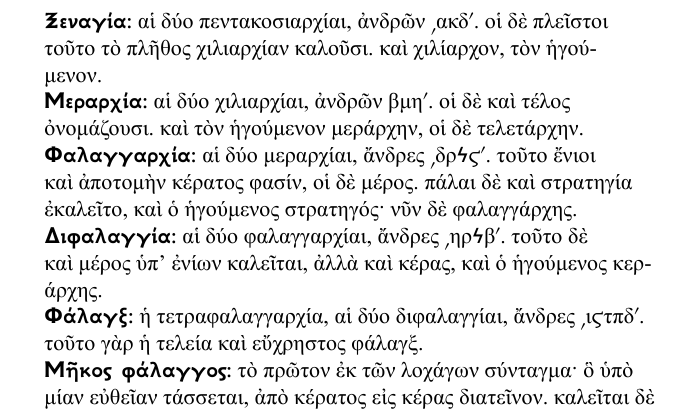
\includegraphics[scale=0.5]{../images/onom-2.png}}
                  \caption{Παράδειγμα αὐτομάτως στοιχειοθετηθέντος
                           κειμένου pdf ἐκ τοῦ Ὀνομαστικοῦ τοῦ
                           Σοῦδα.
                           Ἡ γραμματοσειρὰ εἶναι ἡ Times New Roman ἀλλὰ
                           τὰ ἔντονα γράμματα προέρχονται ἀπὸ τὴν
                           γραμματοσειρὰν GFS Neohellenic.
                           }
                \end{center}
              \end{figure}
  \subsection{Προαιρέσεις στοιχειοθεσίας (Options)}
    Προαιρέσεις αἵτιναι δὲν ἰσχύουν ἀποκτοῦν φαιὰν ὄψιν καὶ παραμένουν
    ἀνενεργαί.\footnote{Ἂν πιέσωμεν ἐπὶ τῆς διακεκομμένης γραμμῆς τοῦ
    ἐπιλογέως, τότε αὐτος ἀποσχίζεται καὶ παραμένει μονίμως διαθέσιμος
    ἐπὶ τῆς ἐπιφανείας.}
    \begin{itemize}
      %
      \item {\bf Author Info:} Παραθέτει λεπτομέρειες περὶ τοῦ κειμένου/συγγραφέος.
      %
      \item {\bf Marginalia: } Ἐὰν τὸ κείμενον ἔχη σημειώσεις
        περιθωρίου θὰ τυπωθοῦν εἰς τὸ δεξιὸν περιθώριον. Ἡ προαίρεσις αὕτη
        ἰσχύει μόνον ἐὰν τὸ κείμενον ἔχη τέτοιες σημειώσεις.
      %
      \item {\bf Citations: } Τὰ τμήματα τῶν κειμένων (βιβλίον, κεφάλαιον,
        παράγραφος κ.λπ.) ἔχουν ἀριθμημένες καταχωρίσεις. Ἡ ἐπιλογὴ αὐτὴ
        ἐμφανίζει ὅλες τὶς ἀριθμήσεις εἰς τὸ ἀριστερὸν περιθώριον ὑπὸ τὴν
        μορφήν: νν.νν.νν.  Ἡ σημασία τῶν ἀριθμῶν αὐτῶν καταδεικνύεται
        κάτω δεξιὰ τοῦ πίνακος τῶν ἔργων τοῦ συγγραφέως.
      %
      \item {\bf \S\ :} Προσθήκη αὔξοντος ἀριθμοῦ κεφαλαίου/παραγράφου
        εἰς τὸ ἀριστερὸν περιθώριον.
        Ἂν τὸ κείμενον περιέχη ἀριθμημένα κεφάλαια/παραγράφους θὰ ὑπάρχη
        ἔνδειξις κάτω δεξιὰ τοῦ πίνακος τῶν ἔργων τοῦ συγγραφέως.
      %
      \item {\bf Line Numbers:} Προσθήκη αὔξοντος ἀριθμοῦ στίχου εἰς τὸ δεξιὸν
        περιθώριον διὰ κάθε πέμπτον στίχον.
      %
      \item {\bf Ligatures:} Στοιχειοθεσία συντομογραφιῶν. Ἐλάχισται
        γραμματοσειραὶ διαθέτουν λιγατοῦρες και συντομογραφίες. Παράδειγμα
        τέτοιας γραμματοσειρᾶς εἶναι ἡ Φιλοκαλία.
      \item {\bf Page Numbers:} Ἀραβική, Λατινικὴ ἢ Ἑλληνικὴ ἀρίθμησις σελίδων.
    \end{itemize}
    \begin{figure}[htb]
      \begin{center}
        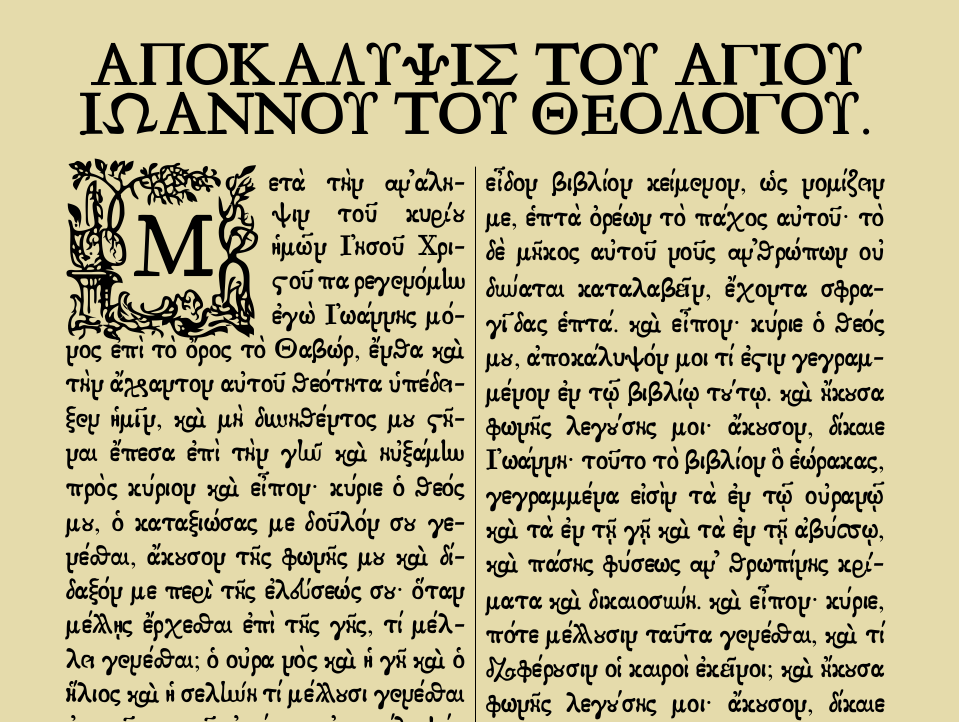
\includegraphics[scale=0.3]{../images/apok.png}
        \caption{Κείμενον στοιχειοθετηθὲν μὲ τὴν
                   προαίρεσιν {\bf Ligatures} καὶ τὴν γραμματοσειρὰν
                   Φιλοκαλία. Ἡ ἔγχρωμη δίστηλος σελὶς ἐπετεύχθη
                   διὰ μικροαλλαγῶν ἐπὶ τοῦ αὐτομάτως παραχθέντος
                   ἀρχείου κώδικος Latex.}
      \end{center}
    \end{figure}
      %
\newpage
  %%%%%%%%%%%%%%%%%%%%%%
  %       Fonts
  %%%%%%%%%%%%%%%%%%%%%%
  \subsection{Ἐπιλογεὺς γραμματοσειρῶν (Fonts)}
    Τὸ στοιχεῖον {\bf Fonts} ἀνοίγει τὸν ἐπιλογέα τῶν γραμματοσειρῶν.
      \begin{figure}[htb]
        \begin{center}
          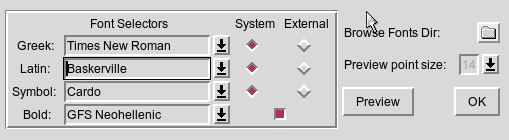
\includegraphics[scale=0.6]{../images/font-selector.png}
          \caption{Ὁ ἐπιλογεὺς γραμματοσειρῶν}
        \end{center}
      \end{figure}
    \paragraph{\bf System Fonts.} Γραμματοσειραὶ ἐγκατεστημέναι ἐν τῶ
      λειτουργικῶ συστήματι ὀνομάζονται {\bf Γραμματοσειραὶ συστήματος}
      (System fonts) καὶ εἶναι διαθέσιμες διὰ τὸν Πρωτέα ὅπως καὶ διὰ
      κάθε ἄλλο πρόγραμμα.
    \paragraph{External Fonts.} Ὁ Πρωτεὺς δύναται νὰ κάμη χρῆσιν καὶ μὴ
      ἐγκατεστημένων, ἤτοι {\bf ἐξωτερικῶν γραμματοσειρῶν} (External fonts).
      Αὗται εἶναι ἀρχεῖα γραμματοσειρῶν τύπου  .ttf~ ἢ .otf
      εὑρισκόμενα εἰς κατάλογόν τινα.\footnote{
              Linux: {\tt /usr/local/proteus/fonts}\newline
              windows: {\tt C:/Program Files/proteus/fonts}
              }\\
      Προσδιορισμὸς/ἀλλαγὴ τοῦ καταλόγου ἐξωτερικῶν γραμματοσειρῶν
      (ἂν ὑπάρχουν) γίνεται διὰ τοῦ κομβίου {\bf Browse Fonts Dir}.

    \vspace{5mm}
    \noindent
    Ἡ στοιχειοθεσία ἑνὸς κειμένου γίνεται καὶ μὲ μίαν μόνον
    γραμματοσειρὰν (π.χ. Times New Roman). Συχνάκις ὅμως
    αἱ γραμματοσειραὶ
    δὲν διαθέτουν ὅλα τὰ ἀπαιτούμενα στοιχεῖα
    ἢ ἂν τὰ διαθέτουν δὲν εἶναι καλαίσθητα. Π.χ. ἡ σειρὰ GFS Didot ἂν
    καὶ ἔχει ἐξαίρετα Ἑλληνικὰ στοιχεῖα, τὰ Λατινικὰ της δὲν εἶναι
    ἀντάξιά τους. Ἕνεκα τούτου ὁ Πρωτεὺς δύναται νὰ ὁρίση
    διαφορετικὰς γραμματοσειρὰς διὰ τὰ Ἑλληνικά, Λατινικὰ
    καὶ τὰ εἰδικὰ σύμβολα.
    Ἡ ἑπιλογὴ γραμματοσειρῶν γίνεται διὰ τῶν τεσσάρων κατιόντων
    ἐπιλογέων γραμματοσειρῶν {\bf Font Selectors}.
    \paragraph{Greek.} Τυπογραφικὰ στοιχεῖα διὰ Ἑλληνικὸν κείμενον.
    \paragraph{Latin.} Τυπογραφικὰ στοιχεῖα μόνον διὰ τὰ Λατινικὰ γράμματα.
    \paragraph{Symbol.}Γραμματοσειρὰ μόνον διὰ τὰ εἰδικὰ σύμβολα, ὅπως
      τὰ Στίγμα (Ϛ), Κόππα (Ϟ), Σαμπὶ (Ϡ), \dag, \ddag\ κ.ἄ.
      Πολλαὶ γραμματοσειραὶ δὲν ἔχουν τὰ εἰδικὰ αὐτὰ σύμβολα.
      Ἔνιαι δὲ γραμματοσειραὶ καίτοι διαθέτουν πολλὰ
      ἐκ των συμβόλων\footnote{Ὄπως λ.χ. αἱ γραμματοσειραὶ Cardo, Libertine
                               κ.ἄ}
      ἴσως νὰ μὴν εἶναι ἐπιθυμηταὶ καθ’ ὅλην τὴν ἔκτασιν τοῦ κειμένου.
    \paragraph{Bold.} Ἐκ τῆς γραμματοσειρᾶς αὐτῆς θὰ γίνει χρῆσις μόνον
      τῶν ἐντόνων στοιχείων της (bold face), ὅπου εἰς τὸ Ἑλληνικὸν κείμενον
      ἀπαιτοῦνται ἔντονα γράμματα. (π.χ. εἰς τὰ λήματα λεξικῶν,
      ὅρα σχῆμα 4.)

      \vspace{3mm}
      \noindent
      Ἀν θέλωμεν μίαν καὶ μόνον γραμματοσειρὰν καθ᾽ ὅλην τὴν ἔκτασιν τοῦ
      κειμένου, τότε ἀπενεργοποιοῦμε
      τὸ bold καὶ θέτωμεν τὴν ἴδιαν γραμματοσειρὰν διὰ τὰ
      Ἑλληνικα, τὰ Λατινικὰ καὶ τὰ σύμβολα.
    \paragraph{Preview.} Παρουσιάζει μικρὸν δεῖγμα
      κειμένου γεγραμμένον εἰς τὰς ἐπιλεγμένας γραμματοσειρὰς πρὸς
      ἐπισκόπησιν πρὸ τῆς ὁριστικῆς
      στοιχειοθεσίας.\footnote{Ἡ προεπισκόπησις εἶναι μόνον διὰ τὰς
                                γραμματοσειρὰς συστήματος.}
      Τὸ μέγεθος τῶν γραμμάτων τῆς προεπισκοπήσεως καθορίζεται διὰ
      τοῦ\linebreak {\bf Preview point size}.
                \begin{figure}[htb]
                  \begin{center}
                    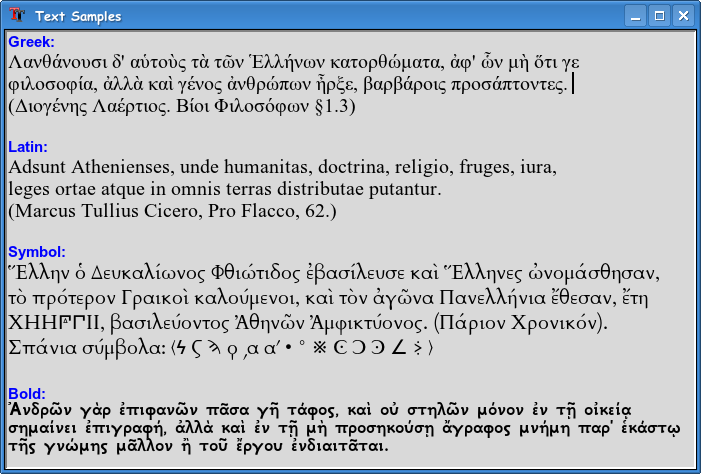
\includegraphics[scale=0.5]{../images/textsamples.png}
                    \caption{Ὁ πίναξ προεπισκοπήσεως γραμματοσειρῶν.}
                  \end{center}
                \end{figure}


\section{Ὀνομασία ἀρχείων}
    Ἡ ψηφιακὴ βιβλιοθήκη περιέχει ἓν ἀρχεῖον ἀνὰ συγγραφέα.
    Ἐπὶ παραδείγματι, τὸ ἀρχεῖον {\bf\tt tlg0012.txt}
    περιέχει τὰ ἅπαντα τοῦ Ὁμήρου.
    Τὸ πρῶτον κατὰ σειρὰν ἔργον ἐν τῶ ἀρχείω εἶναι ἡ Ἰλιάς,
    τὸ δεύτερον ἡ Ὀδύσσεια κ.ο.κ.
    Ἂν λοιπὸν ζητηθῆ ἀπὸ τὸν Πρωτέα νὰ μετατρέψη τὴν Ἰλιάδα,
    θὰ ὀνομάση τὰ παραγόμενα  ἀρχεῖα:
    {\bf {\tt tlg0012\_001.utf}} ἢ {\bf{\tt tlg0012\_001.pdf}}.
    Ὁ κωδικὸς ἀριθμὸς τοῦ ἀρχείου tlg φαίνεται κάτωθεν ἀριστερὰ
    τοῦ καταλόγου τῶν συγγραφέων καὶ ὁ κωδικὸς ἀριθμὸς τοῦ
    ἔργου φαίνεται ἀριστερὰ τοῦ τίτλου.
\section{Εὐχαριστίαι}
    Ἡ ἰδέα τοῦ Πρωτέως γεννήθηκε διαβάζοντας σημειώσεις περὶ beta code,
    Perl καὶ Διογένους τοῦ Peter Hesling δημιουργοῦ
    τοῦ Διογένους.\\
    Ὅρα ἱστότοπον:
    {\tt https://d.iogen.es/d/ }\\*[2mm]

    Τὸ πρόγραμμα C μετατροπῆς ἀπὸ beta code εἰς Unicode
    ἔχει τὶς καταβολές του εἰς τὸ tlgu τοῦ Δημητρίου Μαρινάκη:
    {\tt http://tlgu.carmen.gr/}

\end{document}
